\documentclass{article}


% Language setting
% Replace `english' with e.g. `spanish' to change the document language
\usepackage[english]{babel}

% Set page size and margins
% Replace `letterpaper' with `a4paper' for UK/EU standard size
\usepackage[letterpaper,top=2cm,bottom=2cm,left=3cm,right=3cm,marginparwidth=1.75cm]{geometry}

% Useful packages
\usepackage{amsmath}
\usepackage{graphicx}
\usepackage[colorlinks=true, allcolors=blue]{hyperref}
\usepackage{ocgx}
\usepackage{amssymb}
\usepackage{tikz}

\title{{Algorithms SV worksheet 6}}
\author{Bálint Molnár}

\begin{document}
\maketitle
 


\begin{enumerate}
\item 
Consider a variant of a double-ended queue (deque) that supports the following operations:

\begin{itemize}
    \item \texttt{removeFirst}$(k)$ removes the first $k$ elements from the front of the deque (or clear it if there are less then $k$ elements).
    \item \texttt{add}$(r)$ removes all elements in the deque that are greater than $r$, then inserts $r$ at the end.
\end{itemize}

Design an efficient data structure that supports these operations and analyze their amortized cost.

\item
    Consider an undirected graph with $n$ vertices, where the edges can be coloured blue or white, and which starts with no edges. The graph can be modified using these operations:

\begin{itemize}
    \item \texttt{insert\_white\_edge}$(u,v)$ inserts a white edge between vertices $u$ and $v$.
    \item \texttt{colour\_edges\_of}$(v)$ colours blue all the white edges that touch $v$.
    \item \texttt{colour\_edge}$(u,v)$ colours the edge $u \leftrightarrow v$ blue.
    \item \texttt{is\_blue}$(u,v)$ returns \texttt{True} if and only if the edge $u \leftrightarrow v$ is blue.
\end{itemize}

Give an efficient algorithm that supports these operations, and analyse its amortized cost.

Extend your algorithm to also support the following operation, and analyse its amortized cost:

\begin{itemize}
    \item \texttt{are\_blue\_connected}$(u,v)$ returns \texttt{True} if and only if $u$ and $v$ are connected by a blue path.
\end{itemize}

Extend your algorithm to also support the following operation, and analyse its amortized cost:

\begin{itemize}
    \item \texttt{remove\_blue\_from\_component}$(v)$ deletes all blue edges between pairs of nodes in the blue-connected component containing $v$.
\end{itemize}

\textbf{Note.} It’s easy to gloss over difficulties, so be sure to be explicit about all operations. If you change your data structure to answer a later part, make sure your earlier answers are still complete. This is the sort of question you might be asked in a Google interview; the interviewer will be looking for you to take ideas that you have been taught and to apply them to novel situations.

This question is from Alstrup and Rauhe, via Inge Li Gørt.

\item
You have an island represented by an $N \times M$ grid, with two harbours located on the boundary (either in the first or last row or first or last column). You want to build a border checkpoint line, i.e., a set of cells such that any path between the two harbours must pass through at least one checkpoint cell (a path is a sequence of moves to neighbouring cells, diagonals excluded. Checkpoints cannot be built on harbour cells). Each cell $(i,j)$ has an associated cost $A[i,j]$ to build a checkpoint. 

Find a set of checkpoints satisfying the requirements with minimal cost.

\textbf{Example}

\begin{center}
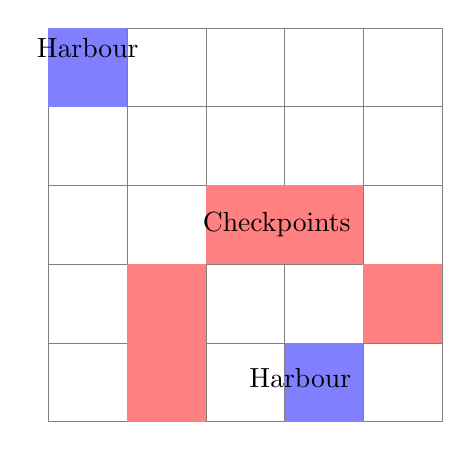
\begin{tikzpicture}
    \draw[step=1cm,gray,very thin] (0,0) grid (5,5);
    
    \foreach \x in {0,...,4} {
        \foreach \y in {0,...,4} {
            \node at (\x+0.5,\y+0.5) {};
        }
    }
    
    % Highlight harbours
    \fill[blue!50] (0,4) rectangle (1,5);
    \fill[blue!50] (3,0) rectangle (4,1);
    
    % Highlight an example checkpoint
    \fill[red!50] (4,1) rectangle (5,2);
    \fill[red!50] (3,2) rectangle (4,3);
    \fill[red!50] (2,2) rectangle (3,3);
    \fill[red!50] (1,1) rectangle (2,2);
    \fill[red!50] (1,0) rectangle (2,1);

    % Labels
    \node[above] at (0.5,4.5) {Harbour};
    \node[below] at (3.2,0.8) {Harbour};
    \node at (2.9,2.5) {Checkpoints};

\end{tikzpicture}
\end{center}

\item
\begin{enumerate}
\item Write a simple pseudocode for polynomial addition and multiplication. What is their time complexity?
    \item 


Prove the following equality for polynomial multiplication:

Given two polynomials:
\[
A(x) = A_0(x) + A_1(x) x^{n}
\]
\[
B(x) = B_0(x) + B_1(x) x^{n}
\]

such that $A_0,A_1,B_0,B_1$ are all polynomials with degree $\leq n$
Show that their product can be computed as:
\[
A(x)B(x) = A_1(x)B_1(x) x^{2n} + ((A_1(x) + A_0(x))(B_1(x) + B_0(x)) - A_0(x)B_0(x) - A_1(x)B_1(x))x^{n} + A_0(x)B_0(x)
\]

\item Use the previous equality to design a divide-and-conquer method for polynomial multiplication that runs in $O(n^{\log_23})$ time (where $n$ is the degree of the polynomials).

\item How would you use this method for multiplying large ($n$-digit) numbers?
\end{enumerate}

\item 

The Travelling Salesman Problem (TSP) is a classic combinatorial optimization problem. Given a set ($V$) of $n$ cities, a ``source'' city $s\in V$ and a distance function $d(i, j)$ that defines the cost of travelling between any two cities $i$ and $j$, the goal is to find the shortest possible route that visits each city exactly once starting from city $s$.
\begin{enumerate}
    \item Write a brute-force method to solve the problem. What is the time complexity of your solution?
    \item Write dynamic programming equations for $\mathrm{DP}(S,v)$ for each $S\subseteq V$ and $v \in V$, where $\mathrm{DP}(S,v)$ is the minimum  cost to visit every city in $S$ starting from $v$. What is the time complexity of the resulting DP algorithm?
    \item Show that the time complexity of the Travelling Salesman problem is $\Omega(n \log n)$. 

    \emph{ Hint: How many branching clauses (e.g. if-else, switch statements etc.) do you need to enter? The argument is similar to the sorting lower bound.}
   
\end{enumerate}
\end{enumerate}

\end{document}

\end{enumerate}
\end{document}